% kate: word-wrap true;

\chapter{Writing System}
\index{Tahano Hikamu|(}

In the previous chapter, example words were given in Ayeri's script, \rayr{thno 
hikmu}{Tahano Hikamu}, wherever possible. Thus, it seems advisable to include a 
description of Ayeri's native writing system here as well. Literally, 
\rayr{thno hikmu}{Tahano Hikamu} means `Round Script' (script round), which is 
an old formation based on the word \xayr{thnF/}{tahan-}{write} that  stuck. The 
current word for `script' is \xayr{thnnF}{tahanan}{writing}. Tahano Hikamu was 
originally named thus because of an earlier draft for a script that never made 
it very far beyond the drawing board and which was a lot more angular, or 
\rayr{hinY}{hinya}, see \autoref{fig:hinya}.\footnote{Unfortunately, there is 
no documentation surviving that I know of.}\index{Tahano Hinya}

\begin{figure}[tp]
\caption{Tahano Hinya and Hikamu}

\begin{minipage}{.5\linewidth}
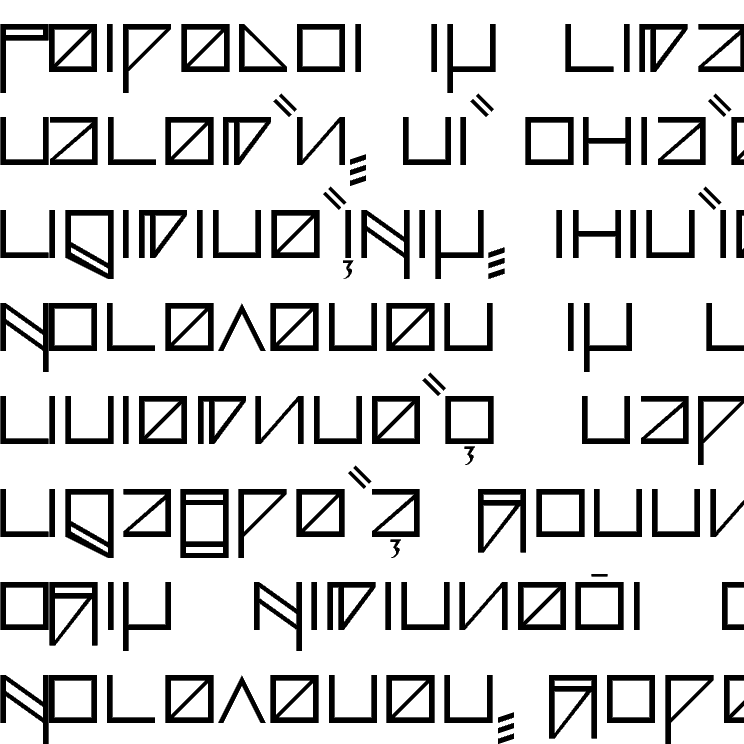
\includegraphics[width=\linewidth]{images/hinya-300dpi-clip.png}
\subcaption{Old and aborted draft: Tahano Hinya}
\label{fig:hinya}
\end{minipage}
~
\begin{minipage}{.5\linewidth}
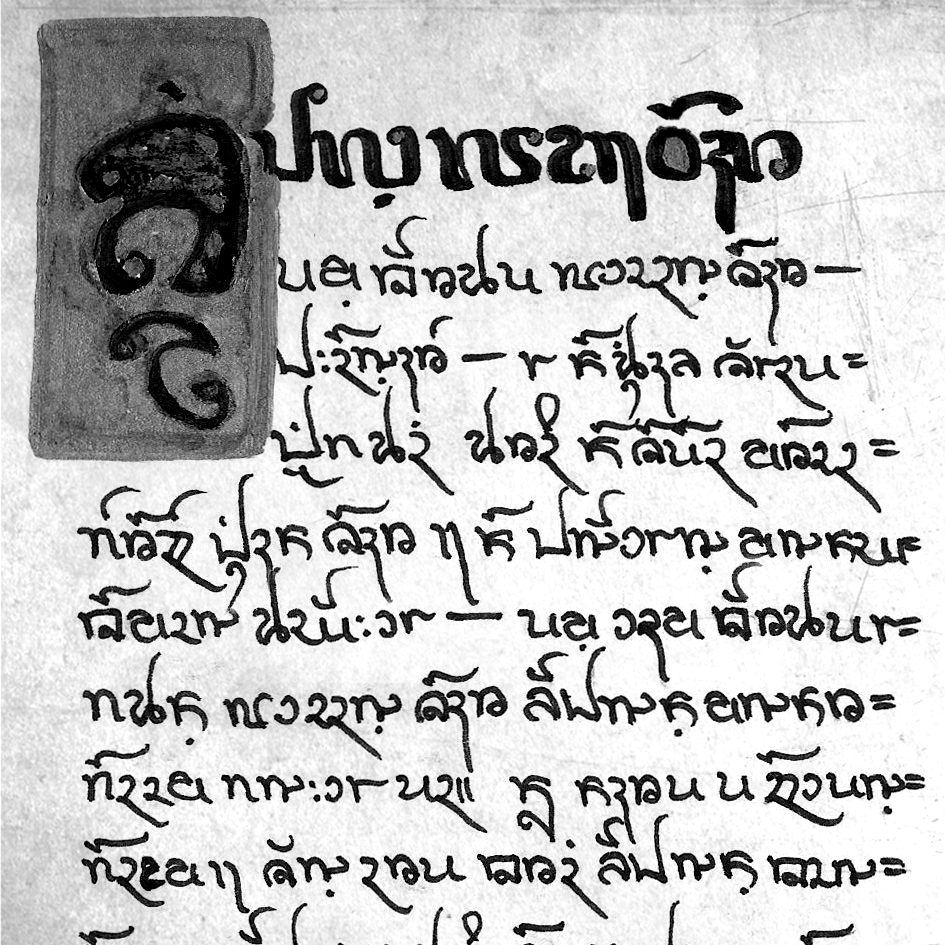
\includegraphics[width=\linewidth]{images/tahano-300dpi-bw-clip.png}
\subcaption{Ayeri's native script: Tahano Hikamu}
\end{minipage}

\label{fig:hinyahikamu}
\end{figure}

As we have seen in the previous chapter, Ayeri's prosody strongly emphasizes 
the syllable as a unit. Thus, it is not a surprise that Ayeri's native script,
Tahano Hikamu, is an alphasyllabary like the Brāhmī-derived alphabets of India 
and Southeast Asia \parencites{salomon1996}{court1996}.\index{Brāhmī scripts} 
This means that its 

\blockcquote[376]{salomon1996}{system is based on the unit of the graphic 
\enquote{syllalbe} […], which by definition always ends with a vowel (type V, 
CV, CCV, etc.). Syllables consisting of a vowel only (usually at the beginning 
of a word or sentence) are written with the \emph{full} or \emph{initial vowel 
signs} […]. But when, as is much more frequently the case, the syllable 
consists of a consonant followed by a vowel, the vowel is indicated by a 
diacritic sign attached to the basic sign for the consonant […].}

For Tahano Hikamu, the definition that a syllable consisting only of a vowel is 
written with an initial vowel sign is only true under certain circumstances, as 
we will see below. Moreover, Brāmī scripts are often characterized by 
conjuncts of clustered consonants which may become quite large and sometimes 
behave in an idiosyncratic way. Consonant conjuncts like Devanāgarī {\FS 
त्व}~\orth{tva} ← {\FS त}~\orth{ta} + {\FS व}~\orth{va} or idiosyncratic 
conjuncts like {\FS क्ष} \orth{kṣa} ← {\FS क} \orth{ka} + {\FS ष} \orth{ṣa} are 
not known in Tahano Hikamu, however. Tahano Hikamu also does not know subscript 
notation for consonant clusters and special diacritics marking coda consonants 
like in Javanese \citep[478--479]{kuipersmcdermott1996}. This does not mean, 
however, that final consonants are simply omitted in writing, since closed 
syllalbes are reasonably common enough to warrant indicating them. Thus, like in 
the Sumatran scripts, there is \textcquote[476]{kuipersmcdermott1996}{a special 
mark to eliminate the vowel of the previous syllable, thereby leaving a 
consonant in a syllable-final position.} That is, there is a diacritic that 
marks the absence of an inherent vowel. With regards to Indian scripts, 
it is referred to as \fw{virāma}; the Ayeri name is 
\xayr{goMdy}{gondaya}{extinguisher}.

Another difference from Brāhmī-family scripts is that all basic vowels have 
unique graphemes; vowel length and diphthongs in [ɪ] are indicated by dedicated 
diacritics. Like in Kharoṣṭhī---another historically important 
ancient script of India---initial vowels are not represented by unique 
graphemes but they are all written like post-consonantal diacritics with the 
grapheme for initial \orth{a} as a basis, \ayr{A} \citep[377]{salomon1996}. The 
\ayr{*a} on \ayr{ʔ} is understood as a diacritic as well, however, namely for 
/a/, which is why it is indicated in the table below as \ayr{ʔ} \orth{Ø} for no 
intrinsic sound value; its native name is 
\xayr{rnYn}{ranyan}{nothing}.\footnote{I will give the native names of graphemes 
here, but will refer to them by their English names for clarity in the 
running text.} Similar to the Javanese script, Tahano Hikamu puts diacritics not 
only below or above consonant bases, but also before them. This, however, is not 
limited to vowel graphemes as in Javanese \citep[478]{kuipersmcdermott1996}.

\section{Consonants}
\index{consonants|(}

Tahano Hikamu is mainly based on consonant bases that are modified by 
diacritics. Since the vowel /a/ is so highly frequent in Ayeri, it is also the 
vowel that is \fw{inherent} to every consonant grapheme if not further modified 
by vowel diacritics. Consonant letters are simply referred to as \textit{pa, ta, 
ka, ...} \autoref{fig:consonants} displays all the main consonants. The 
customary collation is---similar to the IPA table---roughly grouping the letters 
according to their sound value by anteriority (front → back) and sonority (low → 
high). The script is monocameral, that is, there is no distinction between 
capital letters and minuscule letters as in the Latin, Greek, Cyrillic, 
Georgian, and Armenian alphabet. It is also written in lines from left to right.

% \begin{center}\itshape
% 	pa, ta, ka;\\
% 	ba, da, ga;\\
% 	ma, na, nga;\\
% 	va, sa, ha;\\
% 	ra, la, ya;\\
% 	Ø.\\
% \end{center}

\begin{figure}[ht]
\caption{The consonant graphemes of Tahano Hikamu}

\begin{tabu} to \linewidth{X[c] X[c] X[c] X[c] X[c] X[c]}
\toprule
\tableheaderfont	/pa/ & /ta/ & /ka/ & /ba/ & /da/ & /ga/ \\
\rowfont{\Tagati\huge}	p & t & k & b & d & g \\

\midrule

\tableheaderfont	/ma/ & /na/ & /ŋa/ & /va/ & /sa/ & /ha/ \\
\rowfont{\Tagati\huge}	m & n & N & v & s & h \\

\midrule

\tableheaderfont	/ra/ & /la/ & /ja/ & /Ø/ \\
\rowfont{\Tagati\huge}	r & l & y & ʔ \\

\bottomrule
\end{tabu}
\label{fig:thcons}
\end{figure}

What is interesting about \ayr{N}~\orth{nga} is that even though before, /ŋ/ 
was treated strictly as a coda consonant in the previous chapter, it is in fact 
treated as an onset consonant in writing if a vowel is following:

\ex[lingstyle=thex]\begingl
	\gla \ayr{p}	$+$	\ayr{NisF} //
	\glb /pa/	{}	/ŋis/ //
	\glft \rayr{pNisF}{pangis} /paŋ.ɪs/ `money' //
\endgl\xe

Tahano Hikamu knows a few ligatures. First of all, when two \ayr{n} \orth{na} 
are in succession, they will form a ligature \ayr{nn} \orth{nana}:

\ex[lingstyle=thex]\begingl
	\gla \ayr{n}	$+$	\ayr{n}	→	\ayr{nn} //
	\glb /na/	{}	/na/	{}	/nana/ //
\endgl\xe

\noindent This is distinct from conjuncts like in Devanāgarī et al., though, 
since the unmodified sound value will still be /nana/, not */nna/, so the 
inherent vowel of each \ayr{n} \orth{na} is not deleted, and each \ayr{n} 
\orth{na} retains the ability to be modified by diacritics. Tahano Hikamu also 
has a few ligatures of the kind you would find in Brāhmī scripts, however:

\pex
	\a \ayr{q}~\orth{kwa} ← \ayr{k}~\orth{ka} + \ayr{v}~\orth{va},
	\a \ayr{T}~\orth{tsa} ← \ayr{t}~\orth{ta} + \ayr{s}~\orth{sa}, and 
	\a \ayr{x}~\orth{ksa} ← \ayr{k}~\orth{ka} + \ayr{s}~\orth{sa}.
\xe

\noindent These conjunct letters are, however, not normally employed by Ayeri. 
\autoref{fig:thconsadd} shows all additional consonants, added to write other 
languages. Individual languages may adapt the sound values slightly to fit their 
own purposes.

\begin{figure}[ht]
\caption{Additional consonant graphemes of Tahano Hikamu}

\begin{tabu} to \linewidth{X[c] X[c] X[c] X[c] X[c] X[c]}
\toprule
\tableheaderfont	/fa/ & /wa/ & /tsa/ & /za/ & /ʃa/ & /ʒa/ \\
\rowfont{\Tagati\huge}	f & w & T & z & S & Z \\

\midrule

\tableheaderfont	/ça/ & /ksa/ & /kwa/ & /xa/ & /ɣa/ \\
\rowfont{\Tagati\huge}	C & x & q & X & G \\

\bottomrule
\end{tabu}
\label{fig:thconsadd}
\end{figure}

\index{consonants|)}

\section{Vowels}
\index{vowels|(}

As mentioned above, vowels are written as diacritics that are added to 
consonants. In principle, every consonant has two slots for vowels, a primary 
one atop it, and a secondary one below it. Vowels added to consonants in 
the primary slot delete their inherent /a/:

\ex[lingstyle=thex]\begingl
	\gla \ayr{p}	→	\ayr{pe} //
	\glb /pa/	{}	/pe/ //
\endgl\xe

\begin{figure}[th]
\caption{Primary vowel graphemes of Tahano Hikamu}

\begin{tabu} to \linewidth{H[c] X[c] X[c] X[c] X[c] X[c] X[c] X[c]}
\toprule
\tableheaderfont

	& /i/
	& /e/
	& /a/
	& /o/
	& /u/
	& /ə/
	& /aʊ/
	\\
	
\toprule
	
Diaritics
	& \Tagati\huge *i
	& \Tagati\huge *e
	& \huge ({\Tagati *a})
	& \Tagati\huge *o
	& \Tagati\huge *u
	& \Tagati\huge *ə
	& \Tagati\huge *au
	\\

\midrule

Independent
	& \Tagati\huge I
	& \Tagati\huge E
	& \Tagati\huge A
	& \Tagati\huge O
	& \Tagati\huge U
	& \Tagati\huge Ə
	& \Tagati\huge AU
	\\

\bottomrule
\end{tabu}
\label{fig:thvowstop}
\end{figure}

\autoref{fig:thvowstop} gives the primary vowel graphemes. Of the vowel 
graphemes given there, only \ayr{*ə}~\orth{ə} is not used in Ayeri. 
\ayr{*au}~\orth{au} is the only diphthong for which a dedicated grapheme 
exists, even though its occurrence is rather limited. The independent vowel 
graphemes are used at the beginning of words or inside words when there is no 
other way to spell the vowel, which is occasionally the case for secondary 
vowels. Secondary vowels are vowels that are not parts of diphthongs, but follow 
the vowel of a syllable directly. They are attached underneath a consonant base, 
for example:

\ex[lingstyle=thex]\begingl
	\gla \ayr{y}	→	\ayr{ye}	→	\ayr{ye\_a} //
	\glb /ja/	{}	/je/		{}	/je.a/ //
\endgl\xe

In fact, the principle that every consonant base with its diacritics represents 
one syllable is slightly violated here, which is also the reason why secondary 
vowels very occasionally need to be spelled as independent vowels, for example 
when the secondary vowel is long, as in the word \xayr{ruAAnF}{ruān}{duty}:

\ex[lingstyle=thex]\label{ex:rwaa}\begingl
	\gla \ayr{ru}	→	\ayr{ruAA}	\quad	(\,\ayr{ruu\_a}) //
	\glb /ru/	{}	/rwaː/ 		\quad	/ruːa/ //
\endgl\xe

Example (\ref{ex:rwaa}) uses a diacritic, \ayr{*aa}, to indicate length. If 
is put directly under \rayr{ru}{ru} (the \ayr{*\_a} diacritic moves down where 
it is not in the way), the syllable will incorrectly spell /ruːa/ instead of 
the intended /ruaː/. This is because diacritics modify consonants and primary 
vowels, but there is no way to modify a secondary vowel directly. 
\autoref{fig:thvowsbot} gives a list of secondary vowels corresponding to that 
of primary vowels above. The vowels as well are just referred to by their sound 
value; `primary' and `secondary', `superscript' and `subscript' or `upper' and 
`lower' may be chosen to disambiguate their positions; the native names may use 
\xayr{Iraj}{iray}{high} and \xayr{Ejr}{eyra}{low} to disambiguate, so \rayr{E 
Irj}{e iray} denotes the superscript \orth{e} diacritic while \rayr{E Ejr}{e 
eyra} denotes its subscript counterpart.

\begin{figure}[ht]
\caption{Secondary vowel graphemes of Tahano Hikamu}

\begin{tabu} to \linewidth{X[c] X[c] X[c] X[c] X[c] X[c] X[c]}
\toprule
\tableheaderfont	/i/ & /e/ & /a/ & /o/ & /u/ & /ə/ & /aʊ/ \\
\rowfont{\Tagati\huge}	*\_i & *\_e & *\_a & *\_o & *\_u & *\_ə & *\_au \\

\bottomrule
\end{tabu}
\label{fig:thvowsbot}
\end{figure}

As a further exception, those consonant bases with an ascender 
(\ayr{k}~\orth{ka}, \ayr{d}~\orth{da}, \ayr{C}~/ça/) move the primary vowel to 
the secondary slot below the consonant by default while indicating the vacancy 
of the primary slot at the top with a dot. This is done to avoid crossing the 
ascender of the consonant with a vowel diacritic:

\ex[lingstyle=thex]\begingl
	\gla \ayr{k}	→	\ayr{k\_i}	→	\ayr{ki} //
	\glb /ka/	{}	/ka.i/		{}	/ki/ //
\endgl\xe

If the primary vowel slot were not silenced by the \ayr{*\_F} diacritic, it 
could reasonably be assumed that the consonant is not losing its inherent /a/ 
and the vowel below the consonant indicates a secondary vowel, spelling /CaV/. 
If, however, a secondary vowel is \emph{actually} added, primary and secondary 
vowels will be assigned the regular primary and secondary slots, respectively, 
again. This condition also holds true for subscript diacritics.

\pex[lingstyle=thex]
\a\begingl
	\gla \ayr{ki}	→	\ayr{ki\_e} //
	\glb /ki/	{}	/ki.e/ //
\endgl

\a\begingl
	\gla \ayr{ki}	→	\ayr{kii} //
	\glb /ki/	{}	/kiː/ //
\endgl

\xe

The order of secondary vowels and subscript diacritics is iconic insofar as 
it follows the order of sounds in the syllable. Thus, secondary vowels appear 
below the consonant-doubling diacritic, \ayr{*F*}, while they appear above the 
syllable-final homorganic nasal diacritic, \ayr{*\_M}:

\pex[lingstyle=thex]\label{ex:subscrord}
\a\begingl
	\gla \ayr{pFp}	→	\ayr{pFpe\_a} //
	\glb /ppa/	→	/ppea/ //
\endgl

\a\begingl
	\gla \ayr{peM}	→	\ayr{pe\_aM} //
	\glb /peN/	→	/peaN/ //
\endgl
\xe

\index{vowels|)}

\section{Diacritics}
\index{diacritics|(}

We have already encountered two diacritics, one for lengthening the 
primary vowel of a syllalbe and one for deleting the inherent vowel of a 
consonant. Tahano Hikamu comes with a lot more diacritics, however, which 
undergo non-trivial positioning and repositioning rules. As vowels are 
primarily superscripts, diacritics are primarily subscripts, so in the 
following I will first describe subscript diacritics; then preposed diacritics, 
which Ayeri also has a number of, both as graphemes in their own right and as 
allographs of other subscript diacritics; and lastly, superscript diacritics.

\subsection{Subscript Diacritics}

\begin{sidewaysfigure}[p]
\caption{Bottom-attaching diacritics of Tahano Hikamu}
\begin{tabu} to \linewidth{>{\Tagati\huge}X[1] X[8l] X[16l] X[12l]}
\toprule
\tableheaderfont

	& Native name
	& Function
	& Example
	\\
	
\toprule

\tablesubheaderfont\multicolumn{4}{c}{L~a~r~g~e~{ }~d~i~a~c~r~i~t~i~c~s}\\

\midrule

*aa
	& \xayr{tupsti}{tupasati}{long-maker}
	& Lengthens the primary vowel of the syllable
	& \rayr{p}{pa} → \rayr{paa}{pā}
	\\

\midrule
	
*Y
	& \xayr{y Ejr}{ya eyra}{low ya}
	& \orth{ya} following another consonant, also across syllables. Marks 
		palatalization of \ayr{t}~\orth{ta}, \ayr{d}~\orth{da}, 
		\ayr{k}~\orth{ka}, and \ayr{g}~\orth{ga} in Ayeri.
	& \rayr{Ar}{ara} → \rayr{ArY}{arya}; \rayr{t}{ta} → \rayr{tY}{ca}
	\\
	
\midrule
	
*J
	& \xayr{riNy}{ringaya}{raiser}
	& Palatalizes a consonant (not used in Ayeri)
	& \rayr{t}{ta} → \ayr{tJ} /tʲa/, /tʃa/
	\\
	
\midrule
	
*H
	& \xayr{UlNy}{ulangaya}{breather}
	& Aspiration or frication of a consonant (not used in Ayeri)
	& \rayr{t}{ta} → \ayr{tH} /tʰa/, {\addfontfeature{RawFeature=+mgrk}/θa/}
	\\
	
\midrule
	
*\hspace{-.25em}ˀ
	& \xayr{rjpaay Ejr}{raypāya eyra}{low~stopper}
	& Glottal stop coda or glottalization of a consonant (consonant letters 
		with ascenders; not used in Ayeri)
	& \rayr{k}{ka} → \ayr{kQ} /kaʔ/; \rayr{d}{da} → \ayr{dQ} /d’a/
	\\

\midrule

\tablesubheaderfont\multicolumn4{c}{S~m~a~l~l~{ }~d~i~a~c~r~i~t~i~c~s}\\

\midrule

*F
	& \xayr{goMdy}{gondaya}{extinguisher}
	& Deletes inherent /a/ of consonant, e.g. in consonant clusters or 
		closed syllables
	& \rayr{pr}{para} → \rayr{pFr}{pra}, \rayr{prF}{par}
	\\
	
\midrule
	
*M
	& \xayr{vinaati}{vināti}{nasalizer}
	& Indicates a homorganic nasal or nasalizes the vowel, depending on 
		language/context
	& \rayr{pd}{pada} → \rayr{pMd}{panda} /panda/ or /pãda/
	\\
	
\midrule
	
*F*
	& \xayr{kusNisaati}{kusangisāti}{duplicator}
	& Indicates a geminated or otherwise double consonant
	& \rayr{pl}{pala} → \rayr{plFl}{palla}
	\\

\bottomrule
\end{tabu}
\label{fig:thdiabot}
\end{sidewaysfigure}

\autoref{fig:thdiabot} shows the bottom-attaching diacritics. The `large 
diacritics' cause the secondary slot of consonants to move down below the 
diacritic. `Small diacritics' can attach in this place as well as secondary 
vowels, as does the homorganic nasal diacritic \ayr{*M} in this 
diacritic-fraught example:

\ex[lingstyle=thex]\label{ex:caampuluy}\begingl
	\gla \ayr{tYaan} $+$ \ayr{puluj} → \ayr{tYaaMpuluj} //
	\glb {/ˈtʃaːn/} {} {/puˈlʊɪ/} {} {/ˌtʃaːmpuˈlʊɪ/} //
% 	\glc \xayr{tYaanF}{cān}{love} {} \xayr{puluj}{puluy}{opposite} {}
% 		\xayr{tYaaMpuluj}{cāmpuluy}{heterosexual} //
	\glft \xayr{tYaaMpuluj}{cāmpuluy}{heterosexual} //
\endgl\xe

It also needs to be noted that diacritics like \ayr{*Y} are applied to words as 
a whole, not stopping at morpheme and syllable borders, so even though 
\tayr{toryeng}{she sleeps} may be a composed form (\xayr{torF/}{tor-}{sleep} + 
\rayr{/yeNF}{-yeng} (=\TsgF{}.\Aarg{})) and syllabifies as /tor.ˈjeŋ/, the 
spelling is not *\,\ayr{torF\zwsp{}yeNF} as one might expect, but \ayr{torYeNF}.

Even though the primary position for small diacritics is underneath consonants, 
the diacritic deleting the inherent vowel, \ayr{*F}, very commonly also 
appears after a consonant letter at the end of words:

\ex[everygla=\Tagati\Large,everyglb=\itshape]\begingl
	\gla y nimFreN\thafterdot{} pNn\thafterdot{} 
		nraanFyen. //
	\glb Ya nimreng pangan narānyena. //
	\glc Ya nim-reng pangan-Ø narān-ye-na //
	\glc \LocT{} appear=\TsgI{}.\Aarg{} end-\Top{} word-\Pl{}-\Gen{} //
	\glft `It appears at the end of words.' //
\endgl\xe

This strategy is advantageous since Tahano Hikamu leaves very little to no 
space between individual words: \ayr{y nimFreN\thafterdot{} pNn\thafterdot{} 
nraanFyen.} With the dot after the consonant, word boundaries are much more 
visible.

\subsection{Prepended Diacritics}

Example (\ref{ex:caampuluy}) leads us directly to the next class of 
diacritics---ones that are prepended to the consonant letter, either because 
they are simply placed there or because of allography. Let us first list those 
diacritics that appear in front of consonants obligatorily 
(\autoref{fig:thdiapreobl}).

\begin{figure}[htp]
\caption{Obligatorily prepended diacritics of Tahano Hikamu}
\begin{tabu} to \linewidth{>{\Tagati\huge}X[1] X[8l] X[16l] X[12l]}
\toprule
\tableheaderfont

	& Native name
	& Function
	& Example
	\\
	
\toprule

*j
	& \xayr{leMtMkusNF}{lentan\-kusang}{double-\allowbreak{}sound}
	& Marks a diphthong with /ɪ/
	& \rayr{pe}{pe} → \rayr{pej}{pey}
	\\
	
\midrule

*\_:
	& \xayr{tilmy}{tilamaya}{changer}
	& Marks raised vowels (i.e. umlaut; not used in Ayeri)
	& \rayr{po}{po} → \ayr{po\_:}~/pø/
	\\
	
\midrule

*R
	& \xayr{hiymy}{hiyamaya}{roller}
	& Marks retroflex consonants (not used in Ayeri)\footnotemark
	& \rayr{t}{ta} → \ayr{tR}~/ʈa/
	\\

\bottomrule
\end{tabu}
\label{fig:thdiapreobl}
\end{figure}

\footnotetext{In a Tahano Hikamu orthography I devised for English once, 
\ayr{*R} was used for /ɚ/, as in the \textsc{nurse} vowel in American English: 
\rayr{nRsF}{nurse}.}

\begin{figure}[htp]
\caption{Allographically prepended diacritics of Tahano Hikamu}
\begin{tabu} to \linewidth{>{\Tagati\huge}X[1] X[8l] X[16l] X[12l]}
\toprule
\tableheaderfont

	& Native name
	& Function
	& Example
	\\
	
\toprule

ː*
	& \xayr{tupsti mrinF}{tupasati marin}{anterior long-maker}
	& Lengthens the primary vowel of the syllable
	& \rayr{sY}{sya} → \rayr{sYaa}{syā},\newline
		\rayr{n}{na} → \rayr{naa}{nā}
	\\
	
\midrule

ʲ*
	& \xayr{y mrinF}{ya marin}{anterior ya}
	& \orth{ya} following another consonant, also across syllables.
	& \rayr{n}{na} → \rayr{nY}{nya}
	\\
	
	
	& \xayr{riNy mrinF}{ringaya marin}{anterior raiser}
	& Also used as an allograph for the palatalization proper diacritic.
	& \ayr{sH}~/sʰa/ → \ayr{sHY}~/sʰʲ/
	\\
	
\midrule

ʰ*
	& \xayr{UlNy mrinF}{ulangaya marin}{anterior breather}
	& (Pre-)Aspiration or frication of a consonant (not used in Ayeri)
	& \rayr{N}{nga} → \ayr{NH} /ŋʰa/;\newline
		\rayr{t}{ta} → \ayr{ʰt}~/ʰta/
	\\

\bottomrule
\end{tabu}
\label{fig:thdiapreallo}
\end{figure}

As \autoref{fig:thdiapreobl} shows, the only obligatorily prepended diacritic 
that Ayeri uses is the one that marks diphthongs, \ayr{*j}.\index{diphthongs} 
However, there are also a number of diacritics that are also obligatorily 
prepended to consonants, but do so as context-sensitive allographs 
(\autoref{fig:thdiapreallo}). The selection of the variant diacritics is not 
random or up to the aesthetic eye of the writer (even though the device itself 
is certainly a matter of aesthetics), but it is governed by rules. The 
prepended forms listed in \autoref{fig:thdiapreallo} are thus triggered 

\begin{enumerate}
\item when there is no stem or bowl for the regular subscript diacritic to 
	attach to, which is the case for \ayr{n}~\orth{na}, \ayr{N}~\orth{nga}, 
	\ayr{v}~\orth{va}, and \ayr{w}~\orth{wa}:
	
	\begin{multicols}{2}
	\pex[lingstyle=thex,everyglb=\itshape]\label{ex:stemless}
	\a\begingl
		\gla \ayr{n} → \ayr{naa} //
		\glb /na/ {} /naː/ //
	\endgl
	
	\a\begingl
		\gla \ayr{N} → \ayr{Naa} //
		\glb /ŋa/ {} /ŋaː/ //
	\endgl
	
	\a\begingl
		\gla \ayr{v} → \ayr{vaa} //
		\glb /va/ {} /vaː/ //
	\endgl
	
	\a\begingl
		\gla \ayr{w} → \ayr{waa} //
		\glb /wa/ {} /waː/ //
	\endgl
	
	\xe
	\end{multicols}

\item when a large subscript diacritic would be added after another large 
	subscript diacritic---this position can only be filled in once, so 
	further large subscripts are prepended:
	
	\ex[lingstyle=thex,everygla=\normalsize,everyglb=\upshape\Large,
		aboveglcskip=0.5em,numoffset=\leftmargin]\label{ex:stacking}
	\begingl
		\gla {} {$+$ \ayr{*H}} {} {$+$ \ayr{*Y}} {} {$+$ \ayr{*i}} {}
			{$+$ \ayr{*aa}} {} //
		\glb \ayr{t} → \ayr{tH} → \ayr{tHY} → \ayr{tHYi} → 
			\ayr{tHYii} //
		\glc /ta/ {} /tʰa/ {} /tʰja/ {} /tʰji/ {} /tʰjiː/ //
	\endgl\xe
	
	The order of diacritics follows the logic of the respective 
	language's phoneme inventory, so if there are, for example, 
	retroflex consonants and both dental and retroflex consonants can be 
	aspirated, retroflexion would be marked first, then aspiration. If 
	there is a palatalization distinction on top of this, the diacritic 
	would be added after aspiration.
	
	When adding large diacritics to stemless consonants, they are prepended 
	from the beginning, as we saw in (\ref{ex:stemless}), and just like in 
	(\ref{ex:stacking}), this principle continues:
	
	\ex[lingstyle=thex,everygla=\normalsize,everyglb=\upshape\Large,
		aboveglcskip=0.5em,numoffset=\leftmargin]
	\begingl
		\gla {} {$+$ \ayr{*Y}} {} {$+$ \ayr{*aa}} {} {$+$ \ayr{*j}} 
			{} //
		\glb \ayr{n} → \ayr{nY} → \ayr{nYaa} → \ayr{nYaaj} //
		\glc /na/ {} /nja/ {} /njaː/ {} /njaːɪ/ //
	\endgl\xe

\item with consonants directly following \ayr{n}~\orth{na}, to avoid a clash 
	with its swash:
	
	\ex[lingstyle=thex,numoffset=\leftmargin]
	\begingl
		\gla \ayr{n} $+$ \ayr{paa} → \ayr{npaa} \quad
			(*\,\ayr{n\zwsp{}paa}) //
		\glb /na/ {} /paː/ {} /napaː/ {} {} //
	\endgl\xe
	
	An exception to this exception occurs, however, when the consonant is 
	not directly following. In this case, no reordering happens, only 
	\ayr{n}~\orth{na} \emph{may} reduce its descender in size to 
	accommodate the following prepended diacritic:\footnote{The font I am 
	using here is designed so that the reduced combination looks nicer, but 
	if unreduced, \ayr{n}~\orth{na}'s swash is not so long as to cross the 
	descender of \ayr{*j} either.}
	
	\pex[lingstyle=thex,numoffset=\leftmargin]
	\begingl
		\gla \ayr{n} $+$ \ayr{pj} → \ayr{npj} \quad
			(\ques{}\ayr{n\zwsp{}pj}) //
		\glb /na/ {} /paɪ/ {} /napaɪ/ {} {} //
	\endgl\xe
	
\item in other cases where a clash of subscript diacritics needs to be avoided:

	\ex[lingstyle=thex,numoffset=\leftmargin]
	\begingl
		\gla \ayr{di} $+$ \ayr{paa} → \ayr{diːp} \quad 
			(*\,\ayr{dipaa}) //
		\glb /di/ {} /paː/ {} /dipaː/ {} {} //
	\endgl\xe
	
	Alternatively, the following solution is also permissible:
	
	\ex[lingstyle=thex,numoffset=\leftmargin]%
	\begingl
		\gla \ayr{di} $+$ \ayr{paa} → 
		% Due to negligence when coding the Tahano Hikamu font, I did 
		% not build in a way to manually put a diacritic on top of ⟨ka⟩ 
		% and ⟨da⟩, thus I need to put it on the letter with LaTeX 
		% commands, which is very clumsy. Younger self: shame on you!
		\ayr{d\hspace{-.3em}\raisebox{1.5ex}{\zwsp i}\hspace{.3em}%
			paa} //
		\glb /di/ {} /paː/ {} /dipaː/ //
	\endgl\xe
	
	When two long syllables follow each other, as in 
	\tayr{bāmā}{mom-and-dad}, one of the length diacritics should 
	definitely be pulled to the front:
	
	\ex[lingstyle=thex,everyglb=\upshape\Large,
	everyglc=\itshape,aboveglcskip=0.5em,numoffset=\leftmargin]
	\begingl
		\gla {} \ayr{baa} $+$ \ayr{maa} → \ayr{baaːm} \quad 
			(\ques{}\ayr{baamaa}) //
		\glb {\normalsize or:\quad} \ayr{baa} $+$ \ayr{maa} → 
			\ayr{ːbmaa} //
		\glc {} /baː/ {} /maː/ {} /baːmaː/ //
	\endgl
	
	\xe

\end{enumerate}

\subsection{Superscript Diacritics}

Ayeri's standard position for diacritics is below consonants, but sometimes it 
is nicer to put them on top, especially for the letter \ayr{n}~\orth{na} due to 
its swash, as well as for \ayr{v}~\orth{va} since the space below its flag is 
empty otherwise, thus not providing much of a visual connection. The only 
diacritic that is normally attaching at the top of consonants is that for the 
glottal stop---we have already encountered its subscript allograph earlier. 
Since Ayeri's phoneme inventory does not possess a phonemic glottal stop or 
glottalization, this diacritic is not used in Ayeri. The list of superscript 
diacritics is given in \autoref{fig:thdiatop}.

\begin{figure}[htp]
\caption{Superscript diacritics of Tahano Hikamu}
\begin{tabu} to \linewidth{>{\Tagati\huge}X[1] X[8l] X[16l] X[12l]}
\toprule
\tableheaderfont

	& Native name
	& Function
	& Example
	\\
	
\toprule

*\_F
	& \xayr{goMdy liNF}{gondaya ling}{upper extinguisher}
	& Deletes inherent /a/ of consonant, e.g. in consonant clusters or 
		closed syllables
	& \rayr{vr}{vara} → \rayr{v\_Fr}{vra}
	\\
	
\midrule

*\_M
	& \xayr{vinaati liNF}{vināti ling}{upper nasalizer}
	& Indicates a homorganic nasal or nasalizes the vowel, depending on 
		language/context
	& \rayr{nd}{naka} → \rayr{nMk}{nanka} /naŋka/ or /nãka/
	\\
	
\midrule

*̔
	& \xayr{kusNisaati liNF}{kusangisāti ling}{upper duplicator}
	& Indicates a geminated or otherwise double consonant
	& \rayr{pn}{pana} → \rayr{pnFn}{panna}
	\\
	
\midrule

*Q
	& \xayr{rjpaay}{raypāya}{stopper}
	& Glottal stop coda or glottalization of a consonant (not used in Ayeri)
	& \rayr{t}{ta} → \ayr{tQ} /taʔ/;\newline
		\rayr{s}{sa} → \ayr{sQ} /s’a/
	\\

\bottomrule
\end{tabu}
\label{fig:thdiatop}
\end{figure}

While the subscript position is preferred in case of a primary vowel, it may be 
necessary to attach both a superscript diacritic and a vowel sign above a 
consonant. In this case, the consonant-modifying diacritic is placed first and 
the vowel diacritic on top of it---this is exactly equivalent to the rule 
exemplified for subscript diacritics in (\ref{ex:subscrord}).

\index{diacritics|)}

\section{Numerals}
\index{numerals!digits|(}

Ayeri uses a number system based on units of 12, that is, it is duodecimal, 
which is a typological rarity. There is a digit for zero, so the system is 
positional, like the Hindu–Arabic digits used by the Latin alphabet. The numbers 
from 1 to 12 are shown in \ref{fig:thnum}.

\begin{figure}[ht]
\caption{The numerals of Tahano Hikamu}

\begin{tabu} to \linewidth{X[c] X[c] X[c] X[c] X[c] X[c]}
\toprule
\tableheaderfont	0 & 1 & 2 & 3 & 4 & 5 \\
\rowfont{\Tagati\huge}	0 & 1 & 2 & 3 & 4 & 5 \\

\midrule

\tableheaderfont	6 & 7 & 8 & 9 & A & B \\
\rowfont{\Tagati\huge}	6 & 7 & 8 & 9 & ¹ & ² \\

\bottomrule
\end{tabu}
\label{fig:thnum}
\end{figure}

% How are the various mathematical operations indicated, especially the basic 
% ones: addition, subtraction, multiplication, division, equality?

\section{Punctuation and Abbreviations}

...

\index{numerals!digits|)}

\index{Tahano Hikamu|)}
